\chapter{Results}
\label{chap:results}

\section{Visualization and Dimensionality Reduction}
\label{sec:visualization-and-dimensionality}

\subsection{Principal Component Analysis (PCA)}
Principal Component Analysis (PCA) projects the data linearly, preserving the global geometric structure and highlighting the orthogonal ``blocky'' artifacts introduced by the decision-tree-based synthesis \cite{jolliffe2002}. 

\textbf{Normal Distribution}
\begin{figure}[H]
  \centering
  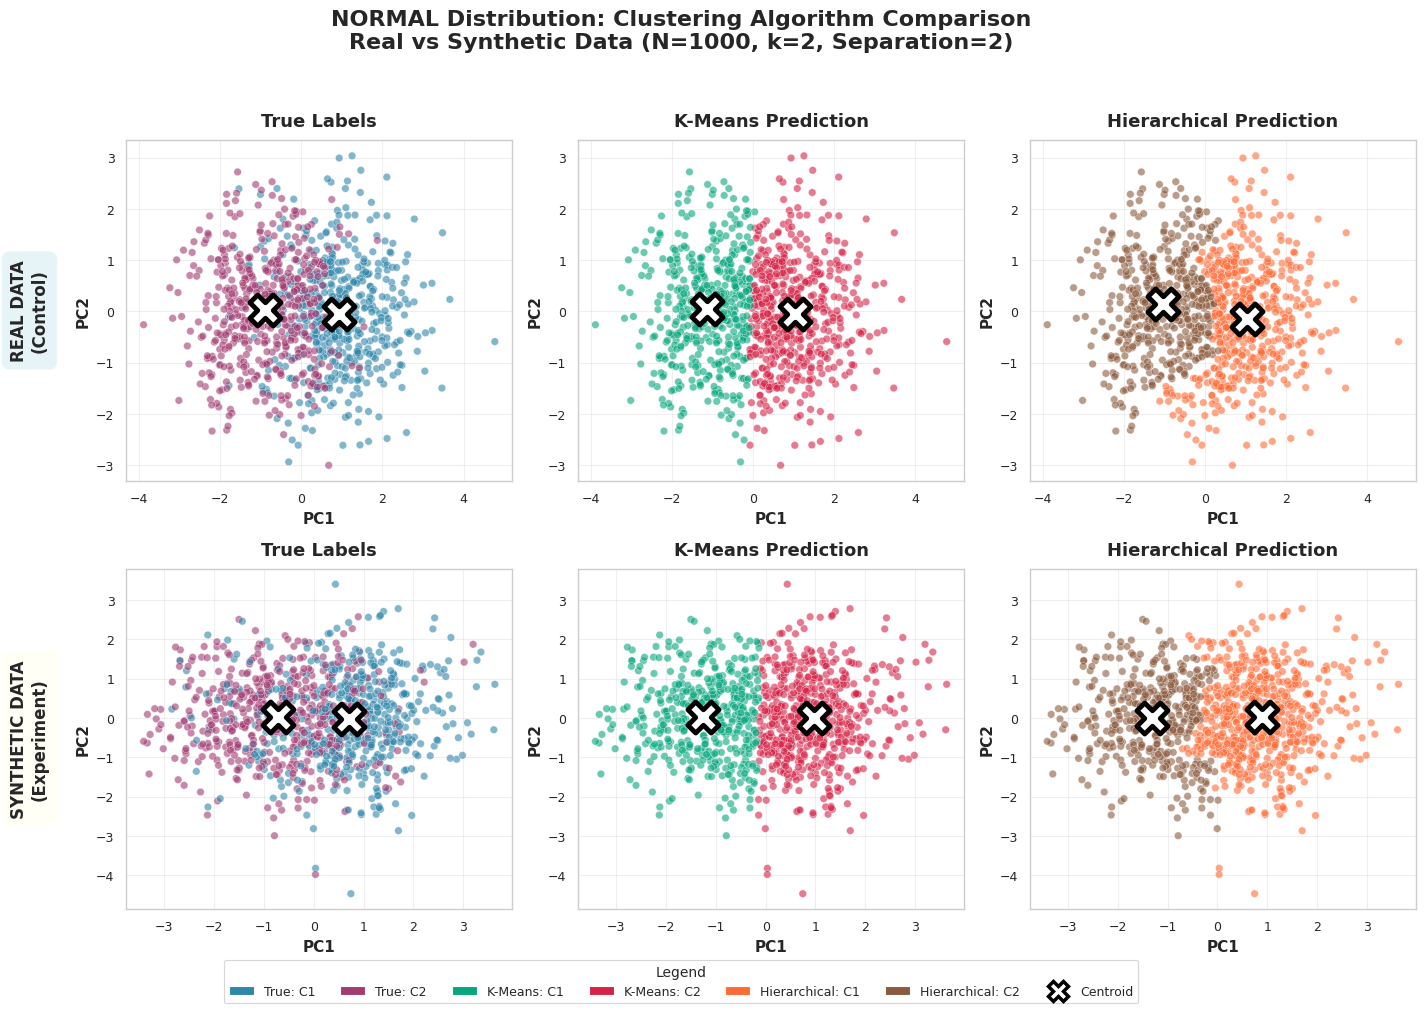
\includegraphics[width=0.9\linewidth]{images/clustering/normal_pca.png}
  \caption{\textbf{PCA Projection: Normal Distribution ($N=1000, k=2$).} Comparison of Real (Top) vs. Synthetic (Bottom).}
  \label{fig:pca_normal}
  \source{Compiled by the author}
\end{figure}

In the Normal distribution case, the spherical nature of the clusters is well-preserved.
\textit{Observation:} The CART synthesis method preserves the spherical geometry of the Normal distribution (Bottom-Left). Consequently, both K-Means and Hierarchical Clustering successfully recover the true cluster labels, demonstrating high utility for normally distributed synthetic data.

\textbf{Gamma Distribution}
\begin{figure}[H]
  \centering
  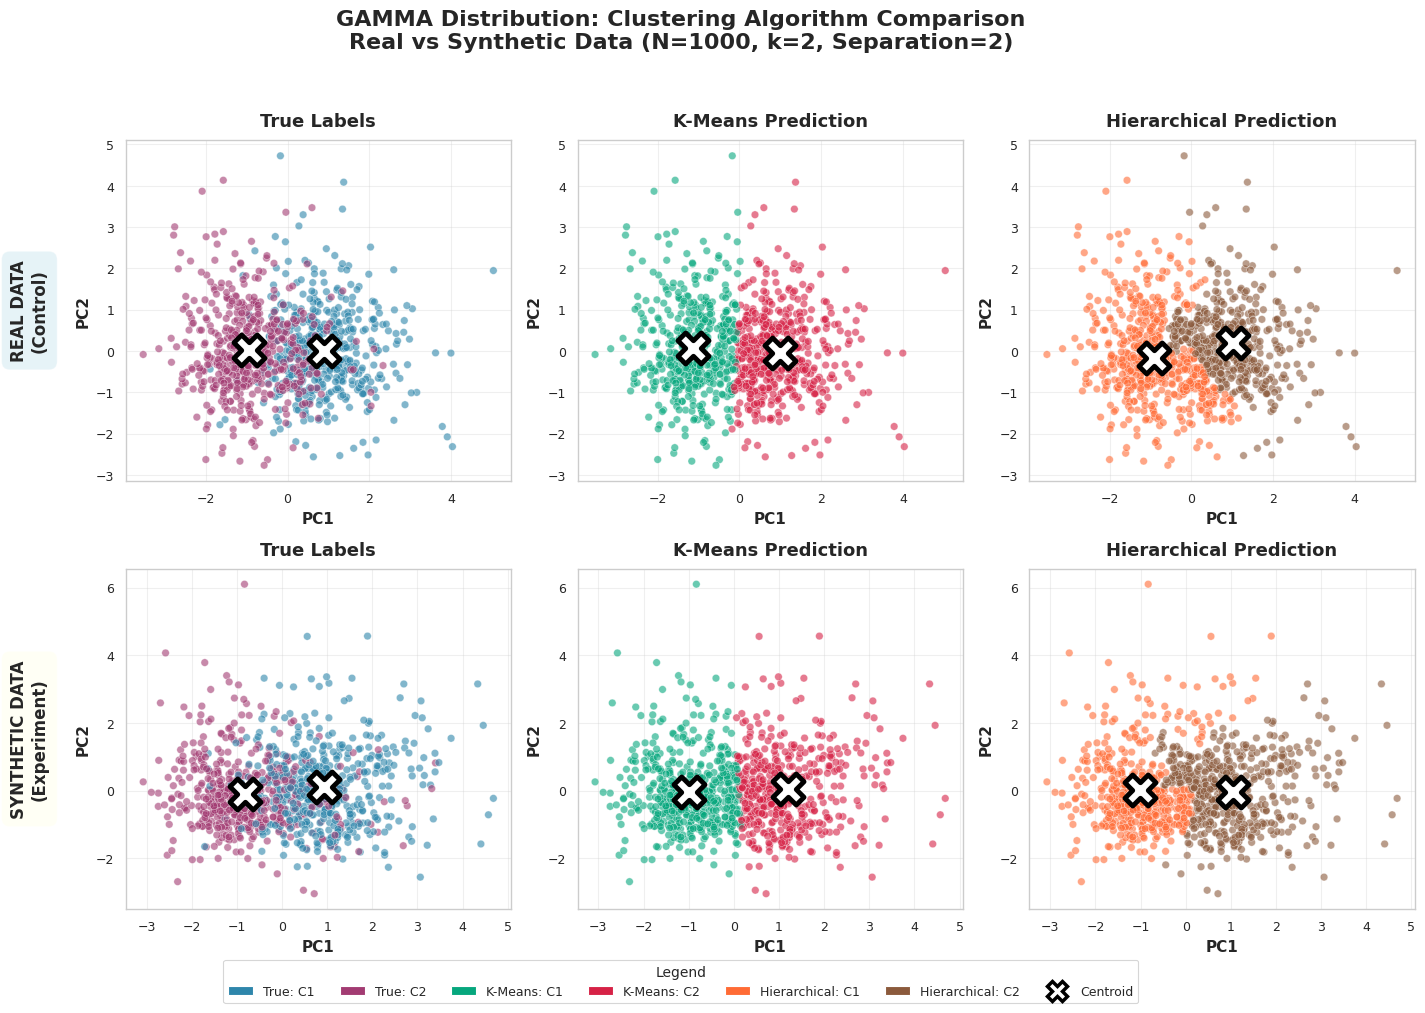
\includegraphics[width=1\linewidth]{images/clustering/gamma_pca.png}
  \caption{\textbf{PCA Projection: Gamma Distribution ($N=1000, k=2$).} Comparison of Real (Top) vs. Synthetic (Bottom).}
  \label{fig:pca_gamma}
  \source{Compiled by the author}
\end{figure}

In the Gamma distribution case, the linear projection reveals the geometric degradation.
\textit{Observation:} The synthetic data (Bottom-Left) exhibits ``hardened'' orthogonal boundaries compared to the smooth tails of the real data. K-Means fails to adapt to this distorted geometry, imposing a linear decision boundary that misclassifies the cluster tails, whereas Hierarchical Clustering proves more robust.

\subsection{t-SNE Analysis}
t-SNE provides a non-linear projection that emphasizes the separation between manifolds \cite{vandermaaten2008}. This visualization is particularly effective at highlighting the ``bad cuts'' made by centroid-based algorithms on skewed data.

\textbf{Normal Distribution}
\begin{figure}[H]
  \centering
  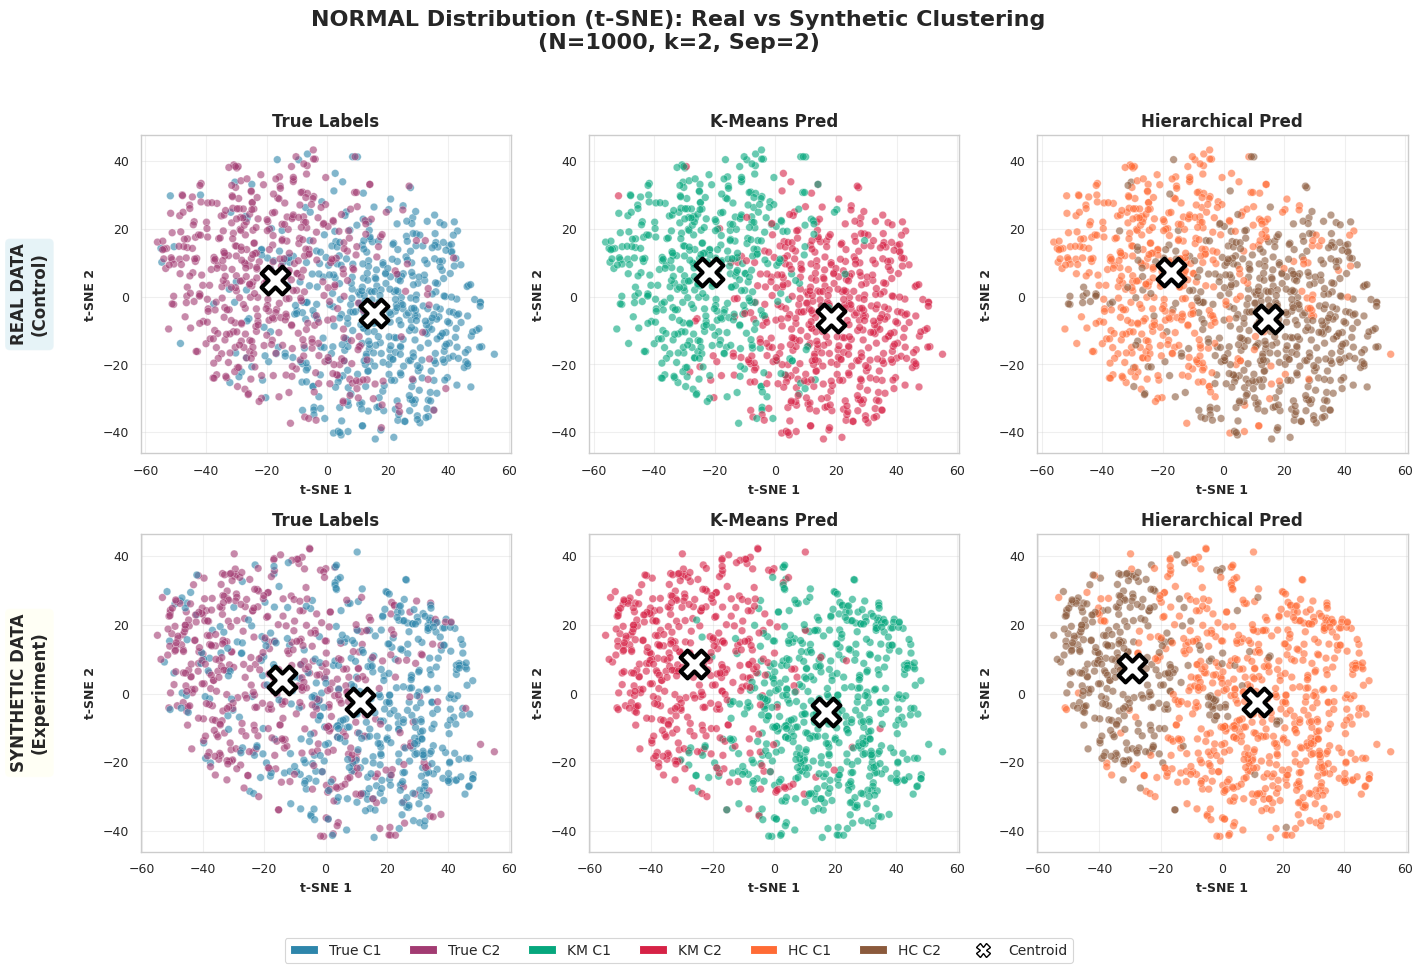
\includegraphics[width=1\linewidth]{images/clustering/normal_tsne.png}
  \caption{\textbf{t-SNE Projection: Normal Distribution.} Comparison of Real (Top) vs. Synthetic (Bottom).}
  \label{fig:tsne_normal}
  \source{Compiled by the author}
\end{figure}

Even in the non-linear projection, the Normal distribution remains cohesive and separable.
\textit{Observation:} The synthetic data (Bottom Row) maintains distinct, separable clusters similar to the control group. Both K-Means and Hierarchical clustering produce nearly identical partitions, confirming that the synthesis process does not introduce topological distortions that affect separability in spherical distributions.

\textbf{Gamma Distribution}
\begin{figure}[H]
  \centering
  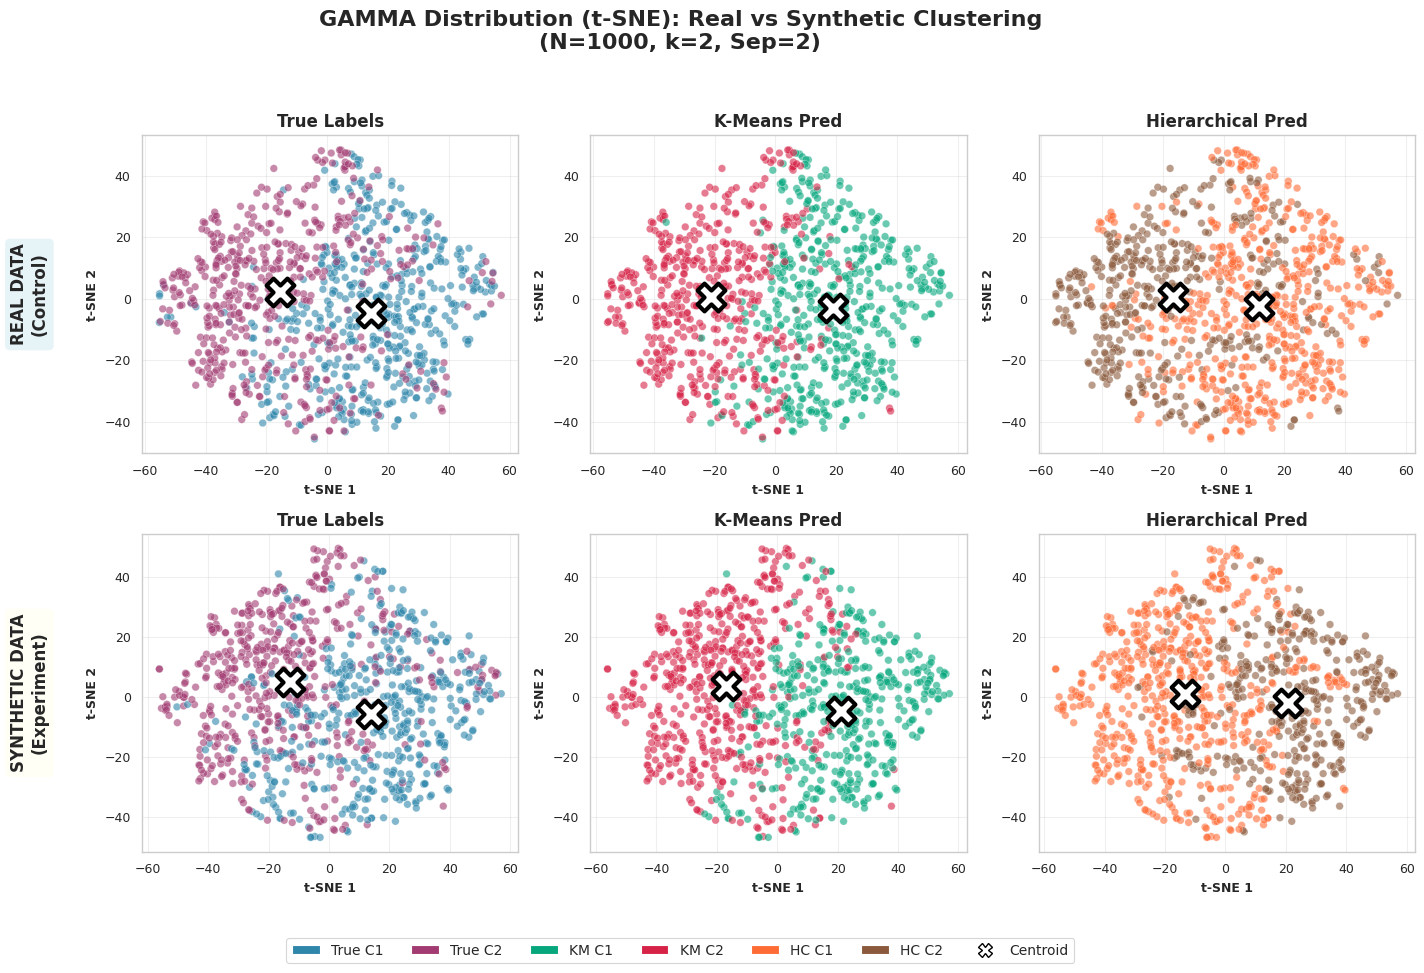
\includegraphics[width=1\linewidth]{images/clustering/gamma_tsne.png}
  \caption{\textbf{t-SNE Projection: Gamma Distribution.} Comparison of Real (Top) vs. Synthetic (Bottom).}
  \label{fig:tsne_gamma}
  \source{Compiled by the author}
\end{figure}

The t-SNE projection reveals the catastrophic failure mode of K-Means on skewed synthetic data.
\textit{Critical Finding:} On synthetic data (Bottom Row), the True Labels show two connected density masses. K-Means (Center) arbitrarily slices these masses with a rigid boundary, failing to capture the organic shape. In contrast, Hierarchical Clustering (Right) successfully identifies the connected structures, offering a significantly closer approximation to the Ground Truth.

\section{Cluster Number Matching}
\label{sec:cluster-number-matching}

This section analyzes the ``Success Rate'' metric---defined as the proportion of synthetic datasets where the algorithm correctly estimated the true number of clusters ($k$). We compare the performance of K-Means and Hierarchical Clustering across varying cluster separations and cluster counts.

For a given configuration with $M$ total simulations, the \textbf{Success Rate (SR)} is calculated as the proportion of correct detections.

\textbf{Normal Distribution}
\begin{figure}[H]
  \centering
  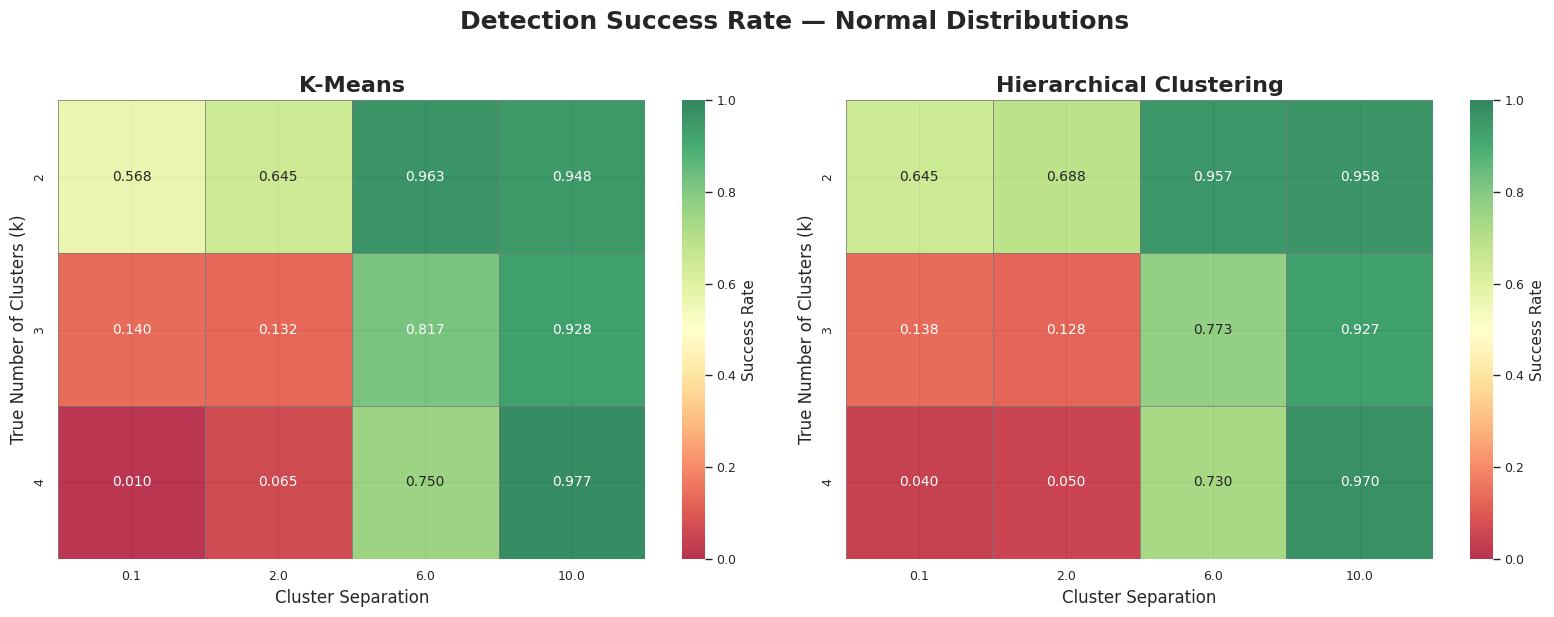
\includegraphics[width=1\linewidth]{images/clustering/dsr_normal.png}
  \caption{\textbf{Success Rate on Normal Distribution.} Left: K-Means. Right: Hierarchical Clustering. Green indicates high success; Red indicates failure.}
  \label{fig:success_normal}
  \source{Compiled by the author}
\end{figure}

\textbf{Observations:}
\begin{itemize}
  \item \textbf{High Separation Stability:} For well-separated clusters, both algorithms achieve near-perfect performance. The synthetic generation artifacts do not hinder detection when the clusters are naturally distinct.
  \item \textbf{Low Separation Degradation:} A sharp performance drop is observed when separation is very low. This suggests that for spherical, overlapping clusters, the ``blocky'' noise from synthetic generation affects both algorithms equally.
  \item \textbf{Algorithm Parity:} In this distribution, the color patterns between K-Means (Left) and Hierarchical Clustering (Right) are largely symmetrical, indicating no significant advantage for either method on spherical data.
\end{itemize}

\textbf{Gamma Distribution}
\begin{figure}[H]
  \centering
  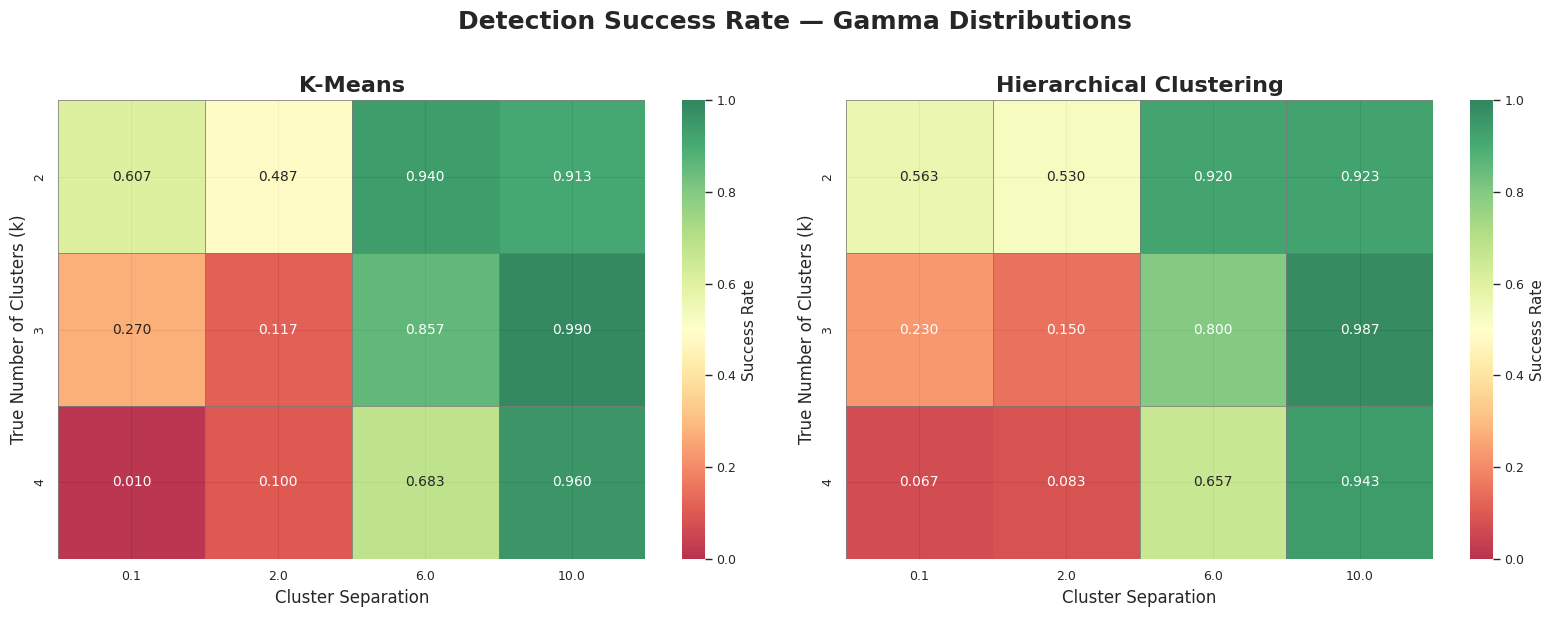
\includegraphics[width=1\linewidth]{images/clustering/dsr_gamma.png}
  \caption{\textbf{Success Rate on Gamma Distribution.} Left: K-Means. Right: Hierarchical Clustering. Note the prevalence of red/orange zones in the K-Means heatmap.}
  \label{fig:success_gamma}
  \source{Compiled by the author}
\end{figure}

\textbf{Observations:}
\begin{itemize}
  \item \textbf{K-Means Collapse:} The K-Means heatmap exhibits a dominant ``Red/Orange'' zone extending into moderate separation levels. Detection is not guaranteed even at higher separations.
  \item \textbf{Hierarchical Robustness:} In contrast, the Hierarchical Clustering heatmap retains significantly more ``Green'' zones, maintaining near-perfect detection while K-Means still shows variability.
  \item \textbf{Performance Delta:} Comparing the two matrices visually reveals a structural divergence. For skewed data, Hierarchical Clustering consistently provides a higher probability of recovering the true $k$, validating its superior handling of the non-linear artifacts introduced by the synthesis process.
\end{itemize}

\section{Gini Coefficient}
\label{sec:gini-coefficient}

To assess structural fidelity, we analyzed the Gini coefficient, which measures the inequality of cluster sizes.

\textbf{Normal Distribution}
\begin{figure}[H]
  \centering
  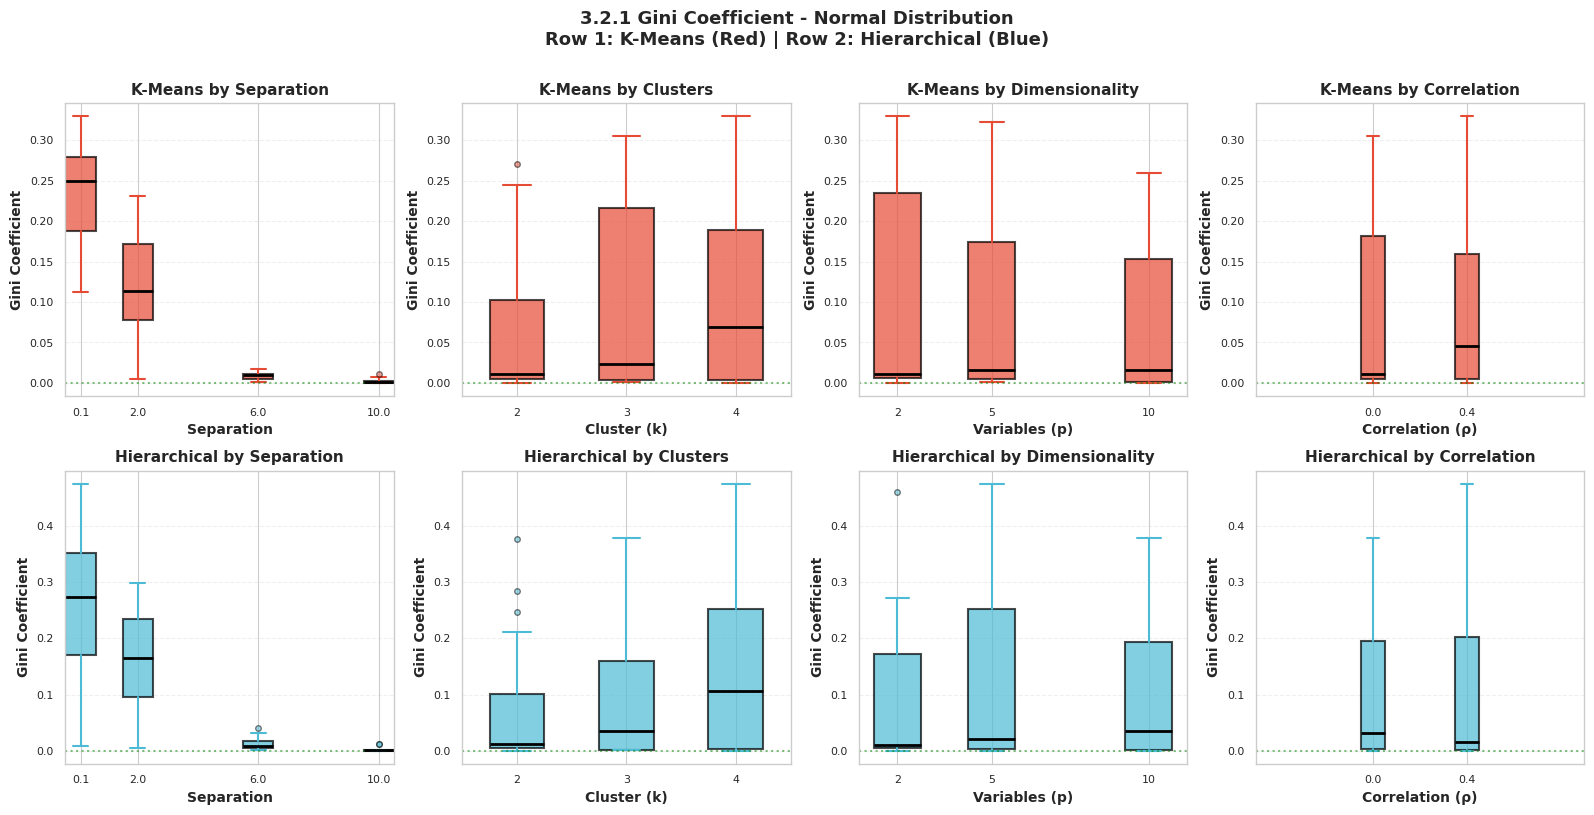
\includegraphics[width=\textwidth]{images/clustering/gini_normal.png}
  \caption{\textbf{Absolute Gini Coefficients (Normal Distribution).} Row 1: K-Means (Red). Row 2: Hierarchical Clustering (Blue). The metric approaches zero as separation increases, indicating balanced detection.}
  \label{fig:gini_absolute_normal}
  \source{Compiled by the author}
\end{figure}

\textbf{Sensitivity to Separation:} Both algorithms exhibit a strong dependency on cluster distinctness. At low separation, the synthetic noise dominates, leading to arbitrary partitions and high imbalance. As separation increases, both algorithms converge to near-perfect balance, confirming that the synthetic generation process does not inherently disrupt cluster balance for well-separated spherical data.

\textbf{Dimensionality Stability:} While K-Means maintains a tight distribution near zero for high dimensions, Hierarchical Clustering exhibits a wider interquartile range and a higher median Gini, suggesting less stability in maintaining balance as feature space grows.

\textbf{Gamma Distribution}
\begin{figure}[H]
  \centering
  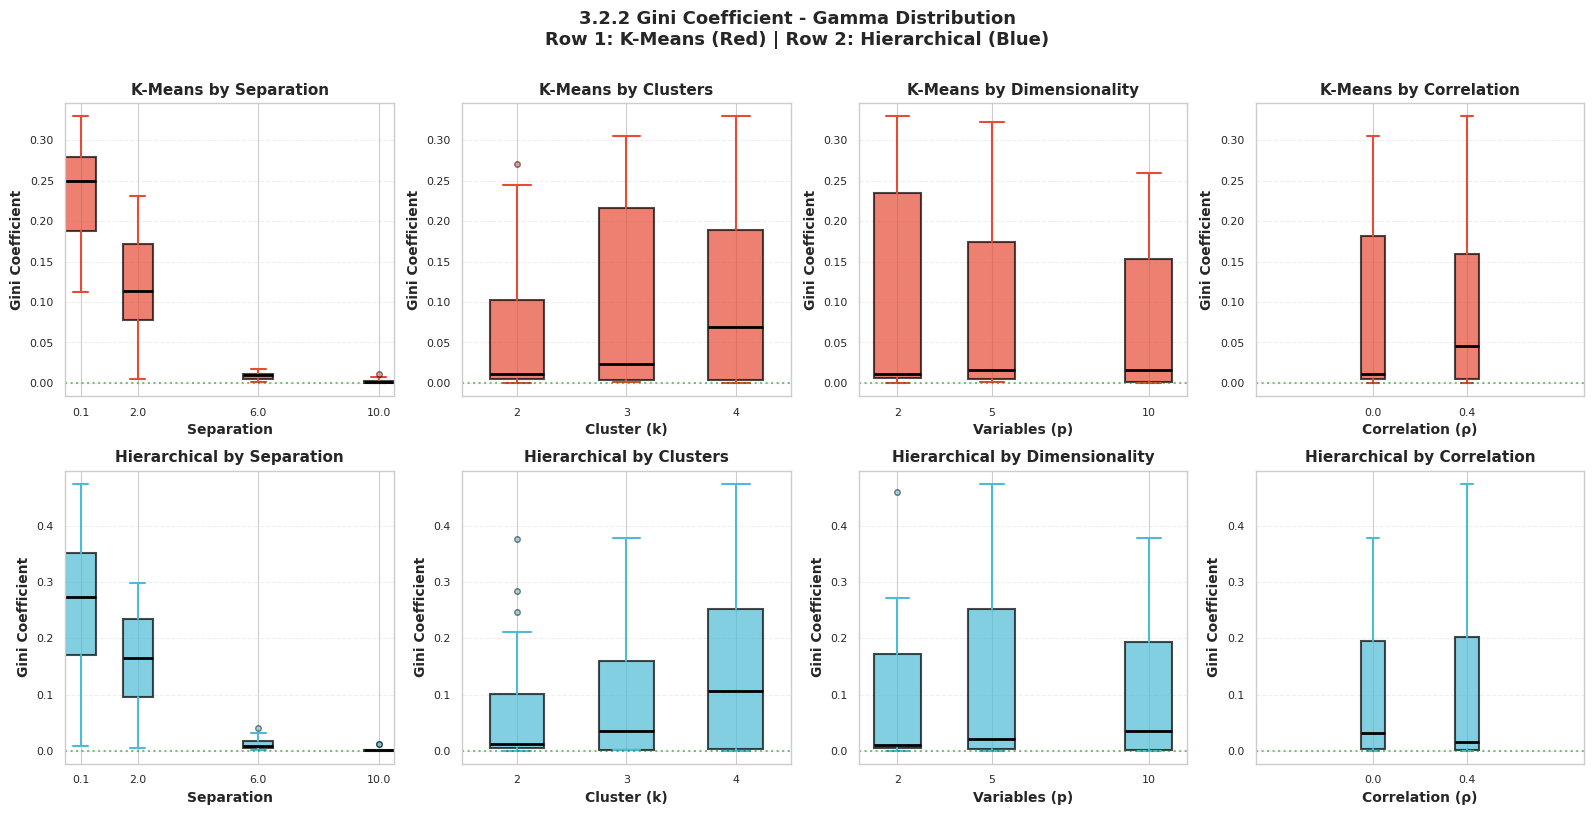
\includegraphics[width=\textwidth]{images/clustering/gini_gamma.png}
  \caption{\textbf{Absolute Gini Coefficients (Gamma Distribution).} Row 1: K-Means (Red). Row 2: Hierarchical Clustering (Blue). Note the high variance in Hierarchical Clustering compared to the rigid stability of K-Means.}
  \label{fig:gini_absolute_gamma}
  \source{Compiled by the author}
\end{figure}

\textbf{K-Means Rigidity:} A striking observation is the consistently low Gini coefficients produced by K-Means. Despite the data being skewed and non-spherical, K-Means minimizes within-cluster variance by imposing a Voronoi tessellation that slices the data into roughly equal volumes. This effectively ``forces'' the skewed data into a balanced structure, suppressing the natural geometric properties of the Gamma distribution.

\textbf{Hierarchical Flexibility (and Instability):} In contrast, Hierarchical Clustering exhibits significantly higher Gini coefficients and wider interquartile ranges. This indicates that Hierarchical Clustering is less constrained by the assumption of equal cluster sizes, allowing it to form imbalanced groups that may better reflect the dense ``heads'' and diffuse ``tails'' of the Gamma distribution, though at the cost of higher variance.

\textbf{Comparative Analysis:} While K-Means remains structurally insensitive to the changing geometry (maintaining a flat, low-Gini profile), Hierarchical Clustering reacts dynamically. This confirms that for non-normal synthetic data, \textbf{K-Means introduces a ``balancing bias''}, while Hierarchical Clustering retains the underlying (imbalanced) structural signal.

\section{Mean Centroid Distance}
\label{sec:mean-centroid-distance}

We computed the Mean Centroid Distance (MCD) to quantify the spatial shift between the cluster centers in the real dataset versus the synthetic dataset.

\textbf{Normal Distribution}
\begin{figure}[H]
  \centering
  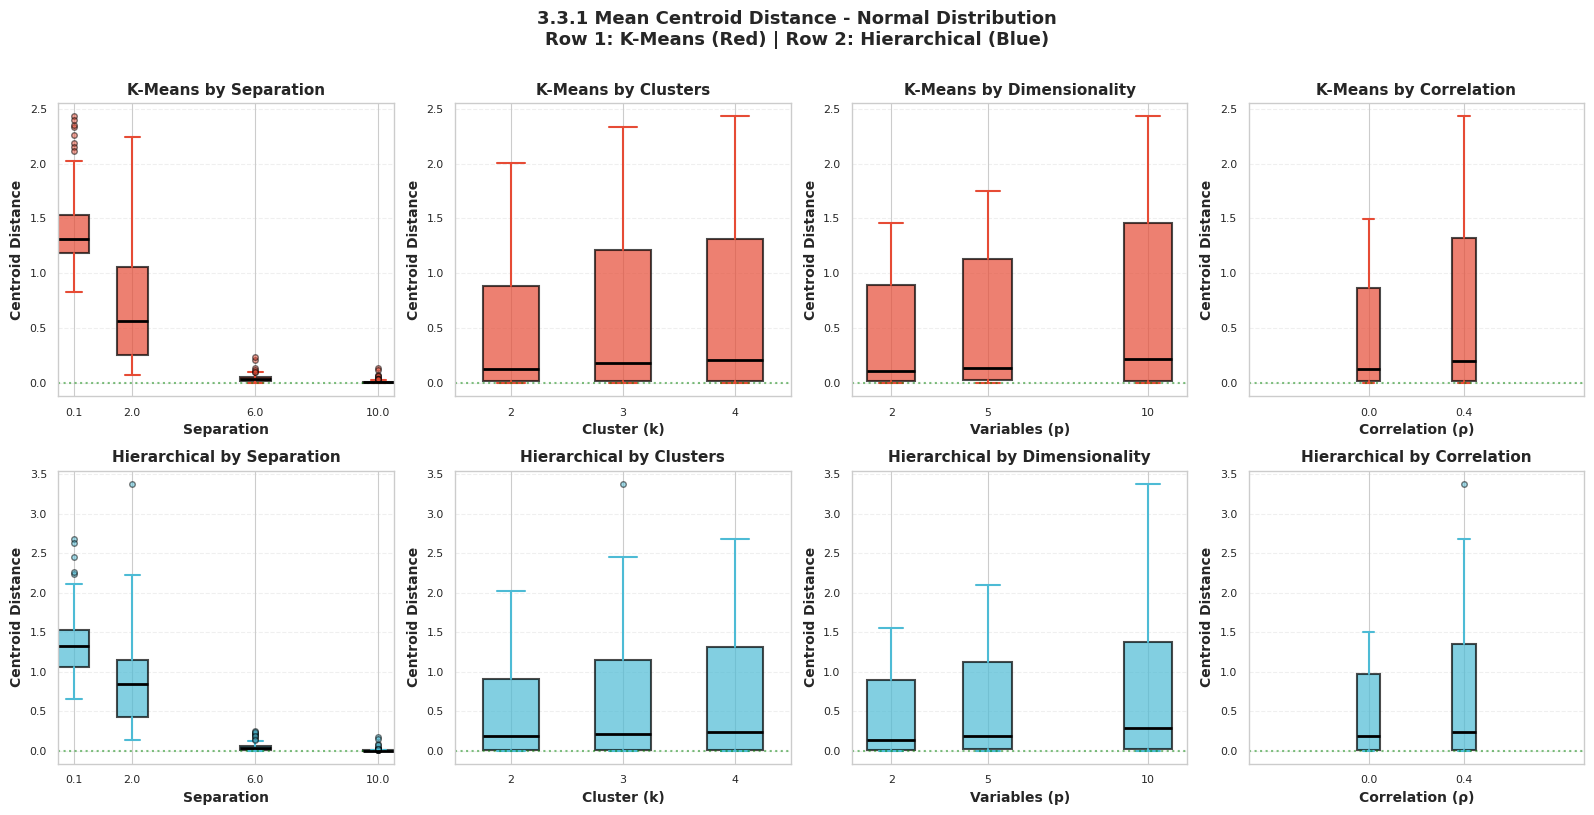
\includegraphics[width=\textwidth]{images/clustering/mcd_normal.png}
  \caption{\textbf{Mean Centroid Distance (Normal Distribution).} Row 1: K-Means (Red). Row 2: Hierarchical Clustering (Blue). The metric quantifies the Euclidean shift of cluster centers after synthesis.}
  \label{fig:mcd_normal}
  \source{Compiled by the author}
\end{figure}

The results show a dominant inverse relationship between cluster separation and centroid stability. At the lowest separation level, both algorithms show high displacement, indicating significant centroid drift when clusters overlap. As separation increases, the distances for both algorithms effectively collapse to zero. In terms of data complexity, the variance of the centroid distance increases with both the number of clusters ($k$) and dimensionality ($p$).

\textbf{Gamma Distribution}
\begin{figure}[H]
  \centering
  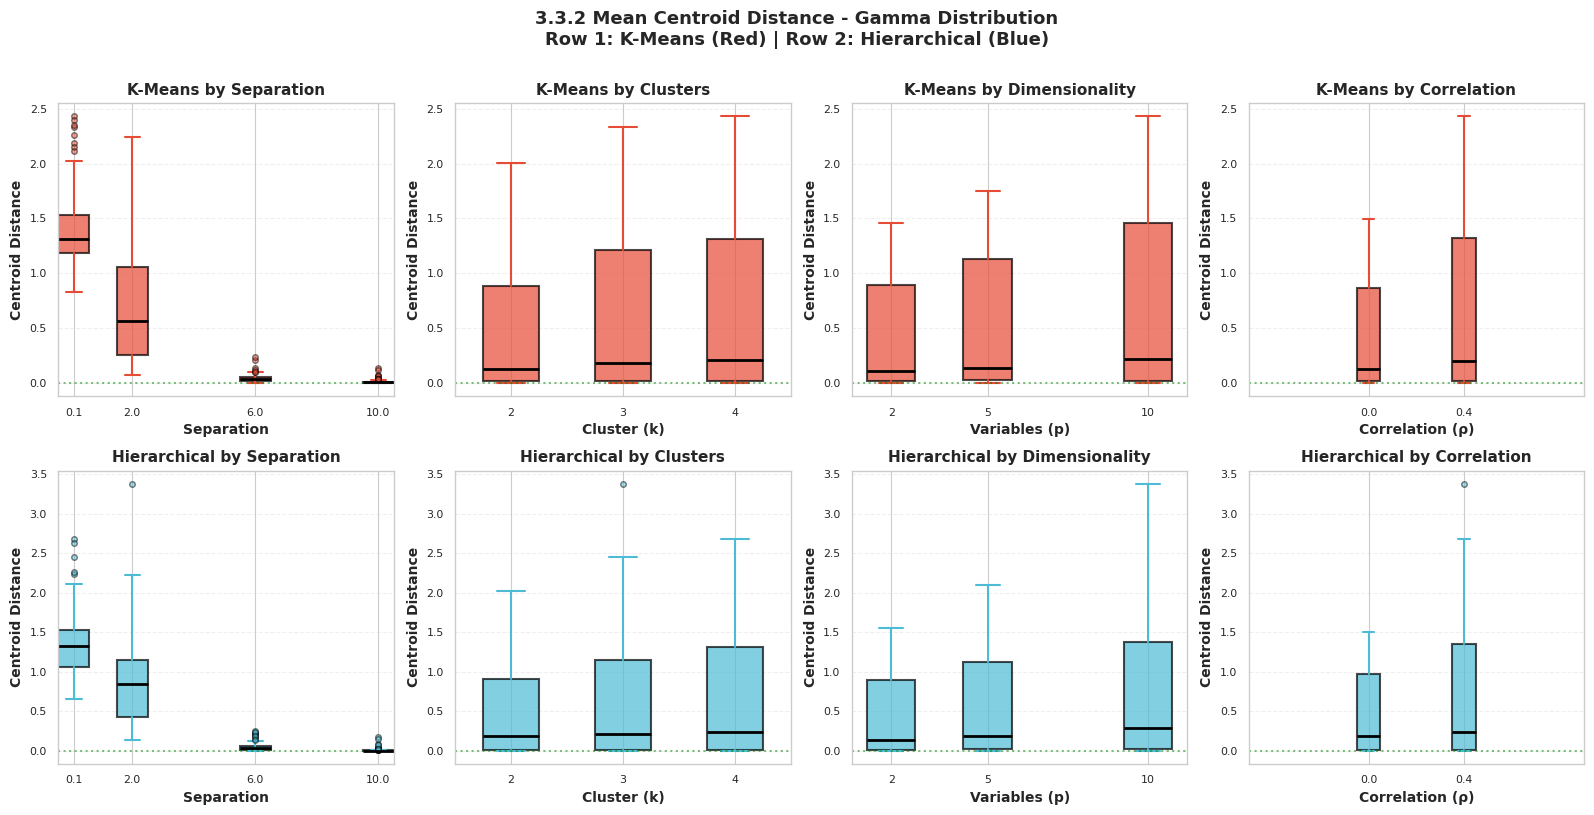
\includegraphics[width=\textwidth]{images/clustering/mcd_gamma.png}
  \caption{\textbf{Mean Centroid Distance (Gamma Distribution).} Row 1: K-Means (Red). Row 2: Hierarchical Clustering (Blue).}
  \label{fig:mcd_gamma}
  \source{Compiled by the author}
\end{figure}

The overall trends closely mirror those observed in the Normal distribution, suggesting that centroid drift is primarily driven by the ``blocky'' artifacts of the CART synthesis method rather than the specific probability distribution. However, the impact of complexity is more pronounced here. Higher dimensionality and a higher number of clusters coincide with increased centroid displacement.

\section{Mean Variance Difference}
\label{sec:mean-variance-difference}

We calculated the Mean Variance Difference (MVD) to measure the discrepancy in within-cluster dispersion between the real and synthetic datasets.

\textbf{Normal Distribution}
\begin{figure}[H]
  \centering
  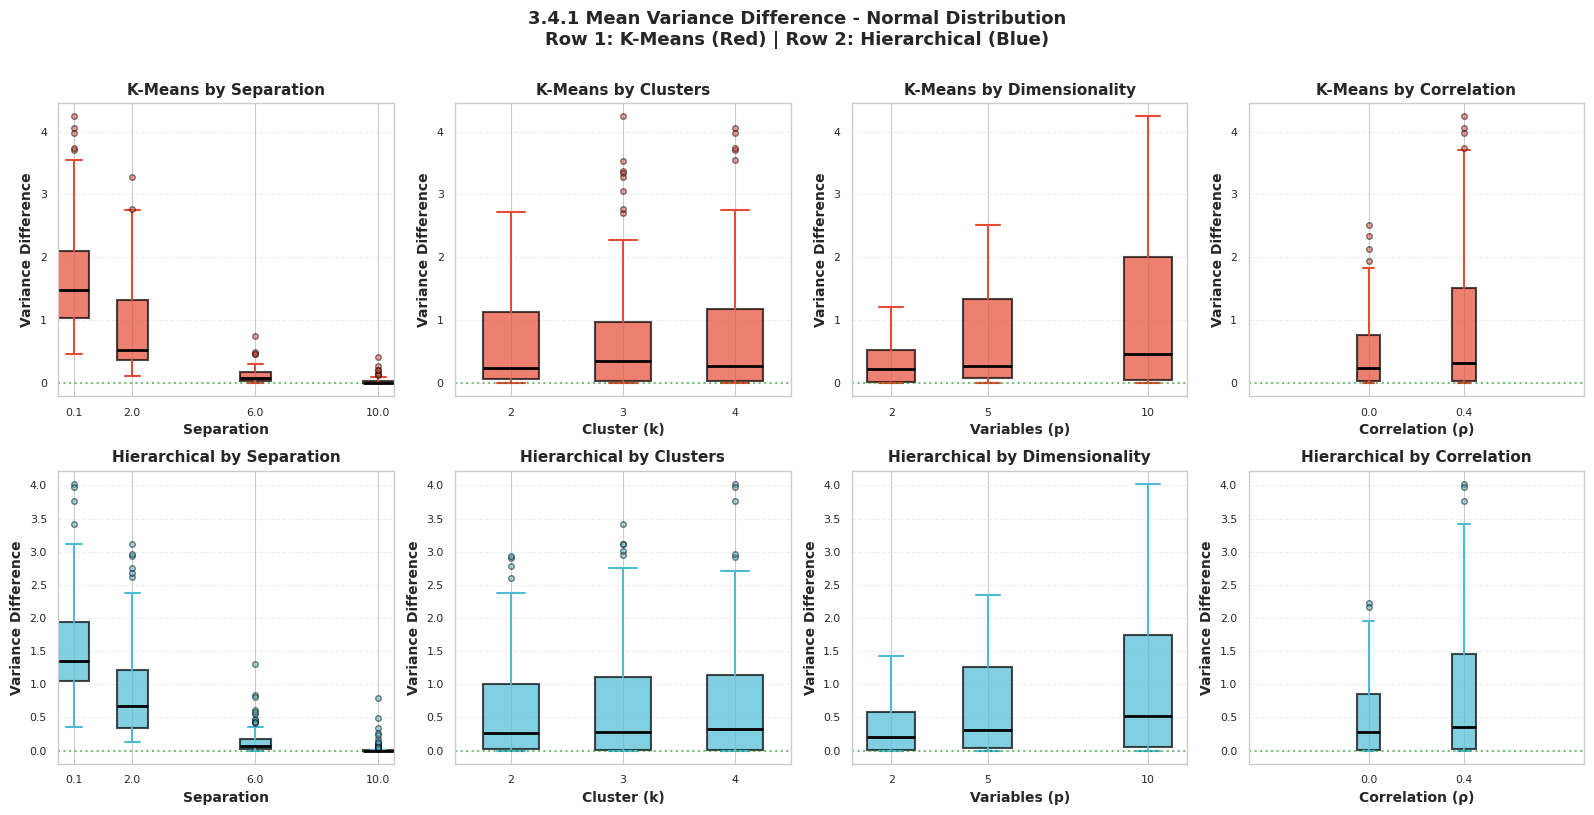
\includegraphics[width=\textwidth]{images/clustering/mvd_normal.png}
  \caption{\textbf{Mean Variance Difference (Normal Distribution).} Row 1: K-Means (Red). Row 2: Hierarchical Clustering (Blue). The metric increases with dimensionality and feature correlation.}
  \label{fig:mvd_normal}
  \source{Compiled by the author}
\end{figure}

The results indicate that cluster separation is the primary factor reducing variance distortion; at high separation, the difference approaches zero for both algorithms. However, structural complexity negatively impacts fidelity. Increasing the number of variables or introducing correlation significantly increases the variance difference. This suggests that the synthetic generation process struggles to replicate the exact dispersion of multivariate normal clusters in higher-dimensional or correlated spaces.

\textbf{Gamma Distribution}
\begin{figure}[H]
  \centering
  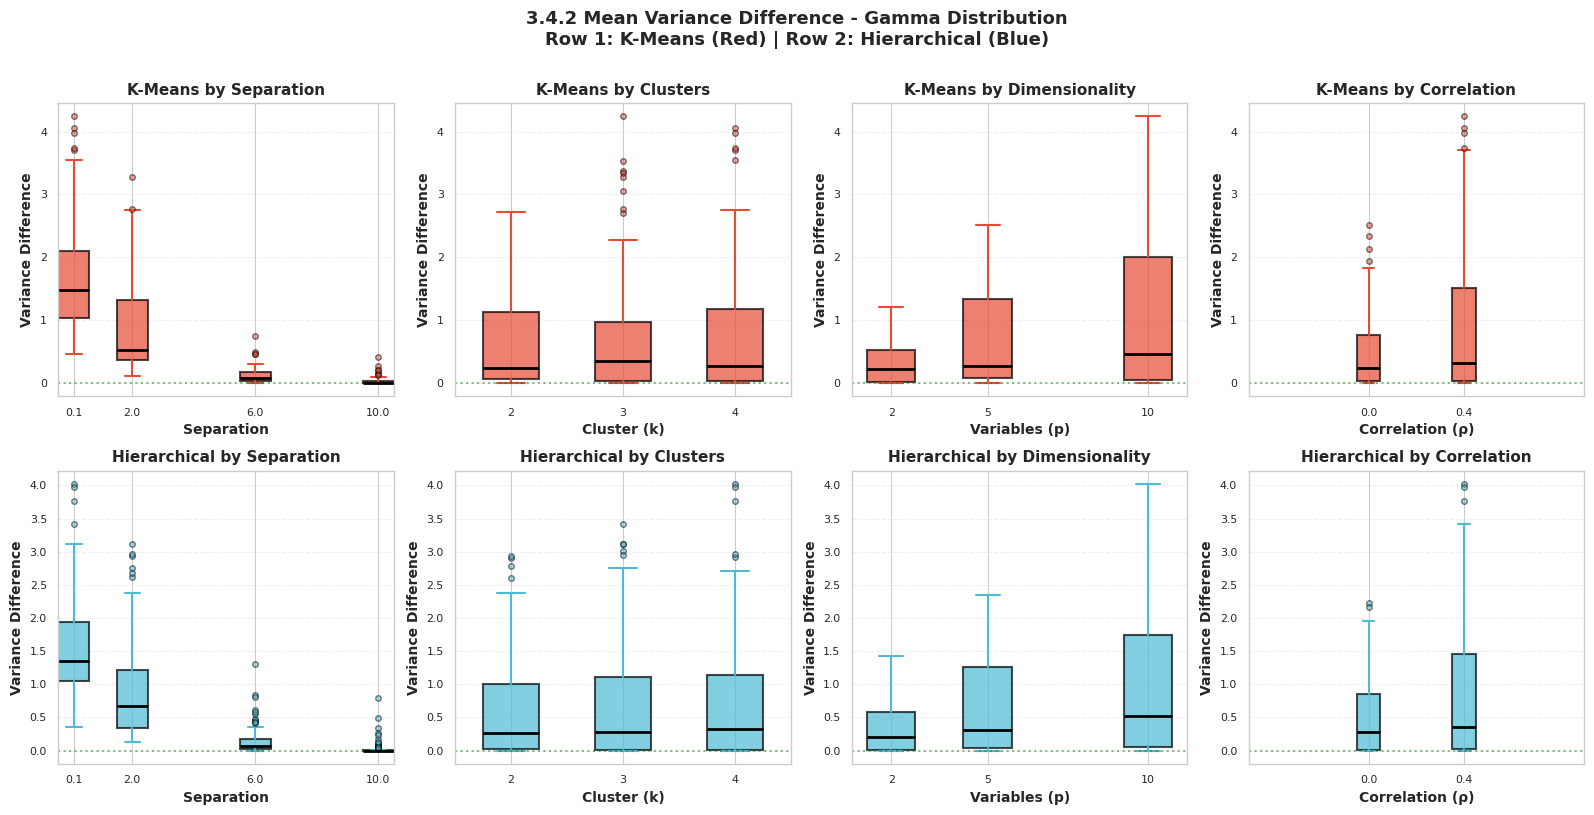
\includegraphics[width=\textwidth]{images/clustering/mvd_gamma.png}
  \caption{\textbf{Mean Variance Difference (Gamma Distribution).} Row 1: K-Means (Red). Row 2: Hierarchical Clustering (Blue). Similar to the Normal case, variance distortion peaks in high-dimensional and correlated settings.}
  \label{fig:mvd_gamma}
  \source{Compiled by the author}
\end{figure}

The variance discrepancy patterns closely track those observed in the Normal distribution, indicating that dispersion artifacts are driven more by the synthetic generation method than the underlying probability distribution. Furthermore, the ``by Dimensionality'' and ``by Feature Correlation'' panels confirm that maintaining accurate cluster variance is increasingly difficult as complexity grows, leading to elevated difference metrics for both algorithms.